%!TEX TS-program = xelatex
\documentclass[11pt]{article}

\usepackage[english]{babel}

\usepackage{amsmath,amssymb,amsfonts}
\usepackage[utf8]{inputenc}
\usepackage[T1]{fontenc}
\usepackage{stix}
\usepackage[scaled]{helvet}
\usepackage[scaled]{inconsolata}

\usepackage{lastpage}

\usepackage{setspace}

\usepackage{ccicons}

\usepackage[hang,flushmargin]{footmisc}

\usepackage{geometry}

\setlength{\parindent}{0pt}
\setlength{\parskip}{6pt plus 2pt minus 1pt}

\usepackage{fancyhdr}
\renewcommand{\headrulewidth}{0pt}\providecommand{\tightlist}{%
  \setlength{\itemsep}{0pt}\setlength{\parskip}{0pt}}

\makeatletter
\newcounter{tableno}
\newenvironment{tablenos:no-prefix-table-caption}{
  \caption@ifcompatibility{}{
    \let\oldthetable\thetable
    \let\oldtheHtable\theHtable
    \renewcommand{\thetable}{tableno:\thetableno}
    \renewcommand{\theHtable}{tableno:\thetableno}
    \stepcounter{tableno}
    \captionsetup{labelformat=empty}
  }
}{
  \caption@ifcompatibility{}{
    \captionsetup{labelformat=default}
    \let\thetable\oldthetable
    \let\theHtable\oldtheHtable
    \addtocounter{table}{-1}
  }
}
\makeatother

\usepackage{array}
\newcommand{\PreserveBackslash}[1]{\let\temp=\\#1\let\\=\temp}
\let\PBS=\PreserveBackslash

\usepackage[breaklinks=true]{hyperref}
\hypersetup{colorlinks,%
citecolor=blue,%
filecolor=blue,%
linkcolor=blue,%
urlcolor=blue}
\usepackage{url}

\usepackage{caption}
\setcounter{secnumdepth}{0}
\usepackage{cleveref}

\usepackage{graphicx}
\makeatletter
\def\maxwidth{\ifdim\Gin@nat@width>\linewidth\linewidth
\else\Gin@nat@width\fi}
\makeatother
\let\Oldincludegraphics\includegraphics
\renewcommand{\includegraphics}[1]{\Oldincludegraphics[width=\maxwidth]{#1}}

\usepackage{longtable}
\usepackage{booktabs}

\usepackage{color}
\usepackage{fancyvrb}
\newcommand{\VerbBar}{|}
\newcommand{\VERB}{\Verb[commandchars=\\\{\}]}
\DefineVerbatimEnvironment{Highlighting}{Verbatim}{commandchars=\\\{\}}
% Add ',fontsize=\small' for more characters per line
\usepackage{framed}
\definecolor{shadecolor}{RGB}{248,248,248}
\newenvironment{Shaded}{\begin{snugshade}}{\end{snugshade}}
\newcommand{\KeywordTok}[1]{\textcolor[rgb]{0.13,0.29,0.53}{\textbf{#1}}}
\newcommand{\DataTypeTok}[1]{\textcolor[rgb]{0.13,0.29,0.53}{#1}}
\newcommand{\DecValTok}[1]{\textcolor[rgb]{0.00,0.00,0.81}{#1}}
\newcommand{\BaseNTok}[1]{\textcolor[rgb]{0.00,0.00,0.81}{#1}}
\newcommand{\FloatTok}[1]{\textcolor[rgb]{0.00,0.00,0.81}{#1}}
\newcommand{\ConstantTok}[1]{\textcolor[rgb]{0.00,0.00,0.00}{#1}}
\newcommand{\CharTok}[1]{\textcolor[rgb]{0.31,0.60,0.02}{#1}}
\newcommand{\SpecialCharTok}[1]{\textcolor[rgb]{0.00,0.00,0.00}{#1}}
\newcommand{\StringTok}[1]{\textcolor[rgb]{0.31,0.60,0.02}{#1}}
\newcommand{\VerbatimStringTok}[1]{\textcolor[rgb]{0.31,0.60,0.02}{#1}}
\newcommand{\SpecialStringTok}[1]{\textcolor[rgb]{0.31,0.60,0.02}{#1}}
\newcommand{\ImportTok}[1]{#1}
\newcommand{\CommentTok}[1]{\textcolor[rgb]{0.56,0.35,0.01}{\textit{#1}}}
\newcommand{\DocumentationTok}[1]{\textcolor[rgb]{0.56,0.35,0.01}{\textbf{\textit{#1}}}}
\newcommand{\AnnotationTok}[1]{\textcolor[rgb]{0.56,0.35,0.01}{\textbf{\textit{#1}}}}
\newcommand{\CommentVarTok}[1]{\textcolor[rgb]{0.56,0.35,0.01}{\textbf{\textit{#1}}}}
\newcommand{\OtherTok}[1]{\textcolor[rgb]{0.56,0.35,0.01}{#1}}
\newcommand{\FunctionTok}[1]{\textcolor[rgb]{0.00,0.00,0.00}{#1}}
\newcommand{\VariableTok}[1]{\textcolor[rgb]{0.00,0.00,0.00}{#1}}
\newcommand{\ControlFlowTok}[1]{\textcolor[rgb]{0.13,0.29,0.53}{\textbf{#1}}}
\newcommand{\OperatorTok}[1]{\textcolor[rgb]{0.81,0.36,0.00}{\textbf{#1}}}
\newcommand{\BuiltInTok}[1]{#1}
\newcommand{\ExtensionTok}[1]{#1}
\newcommand{\PreprocessorTok}[1]{\textcolor[rgb]{0.56,0.35,0.01}{\textit{#1}}}
\newcommand{\AttributeTok}[1]{\textcolor[rgb]{0.77,0.63,0.00}{#1}}
\newcommand{\RegionMarkerTok}[1]{#1}
\newcommand{\InformationTok}[1]{\textcolor[rgb]{0.56,0.35,0.01}{\textbf{\textit{#1}}}}
\newcommand{\WarningTok}[1]{\textcolor[rgb]{0.56,0.35,0.01}{\textbf{\textit{#1}}}}
\newcommand{\AlertTok}[1]{\textcolor[rgb]{0.94,0.16,0.16}{#1}}
\newcommand{\ErrorTok}[1]{\textcolor[rgb]{0.64,0.00,0.00}{\textbf{#1}}}
\newcommand{\NormalTok}[1]{#1}

\newlength{\cslhangindent}
\setlength{\cslhangindent}{1.5em}
\newlength{\csllabelwidth}
\setlength{\csllabelwidth}{3em}
\newenvironment{CSLReferences}[3] % #1 hanging-ident, #2 entry spacing
 {% don't indent paragraphs
  \setlength{\parindent}{0pt}
  % turn on hanging indent if param 1 is 1
  \ifodd #1 \everypar{\setlength{\hangindent}{\cslhangindent}}\ignorespaces\fi
  % set entry spacing
  \ifnum #2 > 0
  \setlength{\parskip}{#2\baselineskip}
  \fi
 }%
 {}
\usepackage{calc} % for \widthof, \maxof
\newcommand{\CSLBlock}[1]{#1\hfill\break}
\newcommand{\CSLLeftMargin}[1]{\parbox[t]{\maxof{\widthof{#1}}{\csllabelwidth}}{#1}}
\newcommand{\CSLRightInline}[1]{\parbox[t]{\linewidth}{#1}}
\newcommand{\CSLIndent}[1]{\hspace{\cslhangindent}#1}\geometry{verbose,letterpaper,tmargin=2.5cm,bmargin=2.5cm,lmargin=2.5cm,rmargin=4.5cm}

\usepackage{lineno}
\usepackage[nolists,noheads]{endfloat}

\pagestyle{plain}

\doublespacing

\fancypagestyle{normal}
{
  \fancyhf{}
  \fancyfoot[R]{\footnotesize\sffamily\thepage\ of \pageref*{LastPage}}
}
\begin{document}
\thispagestyle{empty}
{\Large\bfseries\sffamily The SDM is not the territory: species
distribution models must account for finite abundances}
\vskip 5em

%
\href{https://orcid.org/0000-0002-6506-6487}{M.D.\,Catchen}%
%
\,\textsuperscript{1,2}

\textsuperscript{1}\,McGill University\quad \textsuperscript{2}\,Québec
Centre for Biodiversity Sciences


\textbf{Correspondance to:}\\

\vfill
This work is released by its authors under a CC-BY 4.0 license\hfill\ccby\\
Last revision: \emph{\today}

\clearpage
\thispagestyle{empty}

\vfill
\textbf{\sffamily Abstract: }A representation of a thing is not the same
as that thing.
\vfill

\clearpage
\linenumbers
\pagestyle{normal}

\begin{quote}
Nature does not prepare distributions, only states.

ET Jaynes
\end{quote}

\begin{quote}
I would warn you that I do not attribute to nature either beauty or
deformity, order or confusion. Only in relation to our imagination can
things be called beautiful or ugly, well-ordered or confused

a common misquote of \emph{Baruch Spinoza}, assembled from translated
parts of his \emph{Ethics (Part I)}
\end{quote}

Species do not \emph{actually} have distributions. This may seem a
radical claim, given the rise of species distribution modeling as both a
field of study and imperative for ecosystem management over the last
several decades. But consider that species are composed of discrete
objects---individual organisms that occupy points in space and which
move through time. The location of every individual organism of a
particular species at a particular time is an observable value, which we
could feasibly write down. In most cases the number of individuals of a
species becomes large enough that this is no longer practical.

A distribution is not some inherent property of a given species, but a
conceptual framework that we invoke because we know that sampling of
species locations is incomplete, and in most contexts these location of
the individuals observed in this sample will change as species move
after they are observed. The goal of a species distribution model (SDM)
is instead to take a set of coordinates of observed occurrence of a
species \(\mathbf{O} = \{\vec{o}_1, \vec{o}_2, \dots\}\) and to best
describe a distribution \(D\) such that the true coordinates of the
individuals of that species, denoted
\(\mathbf{X} = \{\vec{x}_1, \vec{x}_2, \dots\}\) are likely to have been
drawn from this distribution \(D\). Note that typically \(|O| \ll |X|\),
as is the reason we don't try to measure the location every individual
in the first place (that being said, for charismatic megafauna that are
nearly extinct, this \emph{is} what we do, precisely because it is
feasible). Yet this should not be mistaken for the distribution \(D\)
being an inherent but latent ``property'' of species.

Many approaches have been taken to design SDMs, but almost universally
the output of an SDM is a raster, where the value of each location/cell
\(i\), denoted \(p_i\), forms a distribution as \(\sum_{i} p(i) = 1\).
The value of a cell is often referred to in plain language as
``occurrence probability.'' But what is meant by this?---is it the
probability conditional on observing an individual that it will be
observed at that location? Or is it the probability that an observer
would find an individual of this species at location if they ``look hard
enough?''

This semantic confusion is a by-product of using a distribution as a
tool to model something that is discrete --- the finite number of
individuals of a species that exist across space. Regardless of the
paradigm used to design the model predicting occurrence probability, the
framing of \emph{occurrence probability} as existing per unit space is
fundamentally a \emph{frequentist} view of probability, as this does not
consider that a finite number of samples from this spatial distribution
are unlikely to produce, and instead imposes the idea of a ``long-run''
probability of occurrences.

. A more appropriate way to view this would be the probability you
observe an individual at a location \(\vec{x}\) as conditional on there
being \(N\) total individuals of a given species across the entire
spatial domain, \(p = P(\vec{x} | N)\)--- we illustrate this using a
``sandbox'' SDM in the next section.

\hypertarget{an-illustration}{%
\section{An illustration}\label{an-illustration}}

What is the value for which \(p(x)\) is non-zero, but \emph{effectively}
\(0\)?

The goal in this section is to determine how the abundance of a species
is \(N\) effects the meaning of the occurrence probability

species all occur in cells of the raster with a probability-value
\(A_{xy}\) that is greater than some threshold. Dare I say it, but this
section may contain multiple integrals.

Consider an SDM where the probability of occurrence of a species is
given for each location \(x\) is given by \(P(x)\). Assume the
rank-frequency distribution values of \(P(x)\) follow an exponential
distribution, with pdf \(f(x) = \lambda e^{-\lambda x}\). What is the
probability that for \(N\) observations of this species, that all of
them occur in cells above some threshold value \(\epsilon\)?

\begin{figure}
\hypertarget{fig:density}{%
\centering
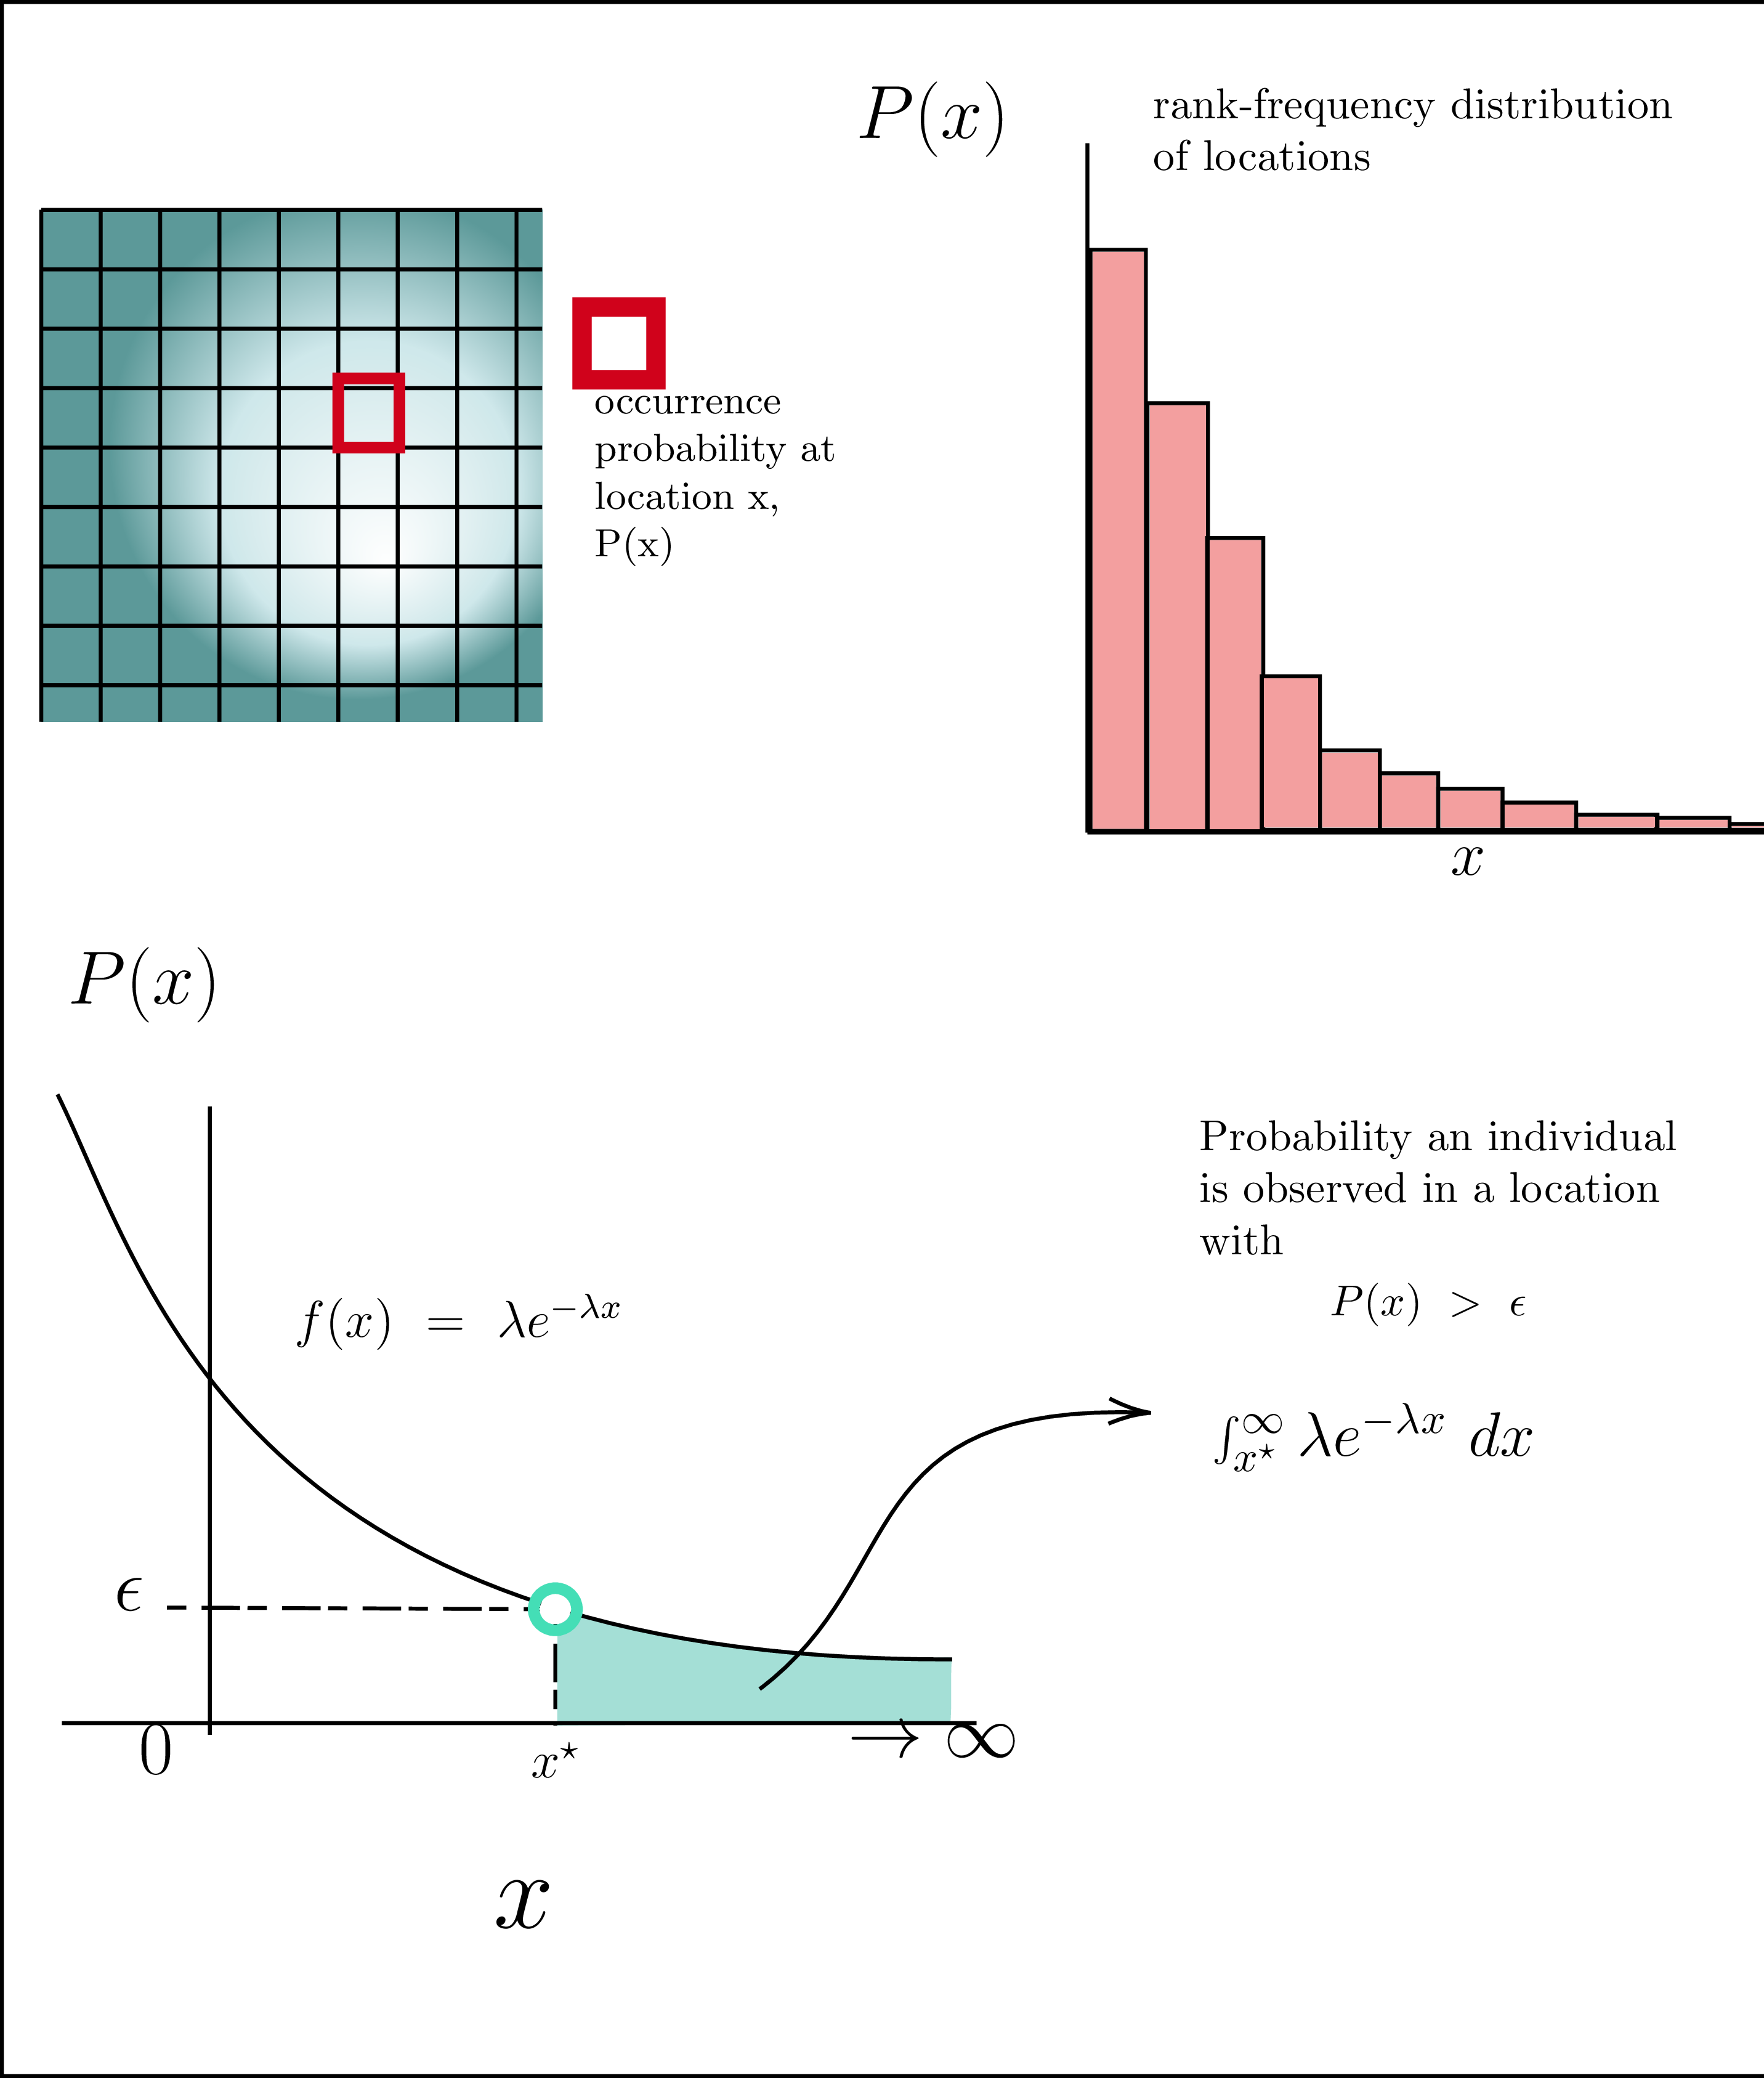
\includegraphics{./figures/probdensity.png}
\caption{todo}\label{fig:density}
}
\end{figure}

We start by determining what the probability of a single observation
happening \emph{below} \(\epsilon\). Assume
\(O \sim \text{Exp}(\lambda)\). Then

\[P(O < \epsilon) = \int_{x^\star}^\infty f(x) dx\]

From this we see \(\epsilon = \lambda e^{-\lambda x^\star}\) which
implies

\[\implies x^\star = \frac{1}{\lambda}\ln \bigg(\frac{\lambda}{\epsilon} \bigg)\]

substituting into first line and integrating, because the exponential
distribution is nice this cosmic gumbo now reduces to

\[P(O < \epsilon) = \frac{\epsilon}{\lambda}\]

Next, we take this result and plug it back into our original question,
which is the probability that none of \(N\) observations occur below
\(\epsilon\) which we can express as

\(\text{Beroulli}\big(N, (1 - \frac{\epsilon}{\lambda})^N\big)\)

which looks like

\begin{figure}
\hypertarget{fig:neato}{%
\centering
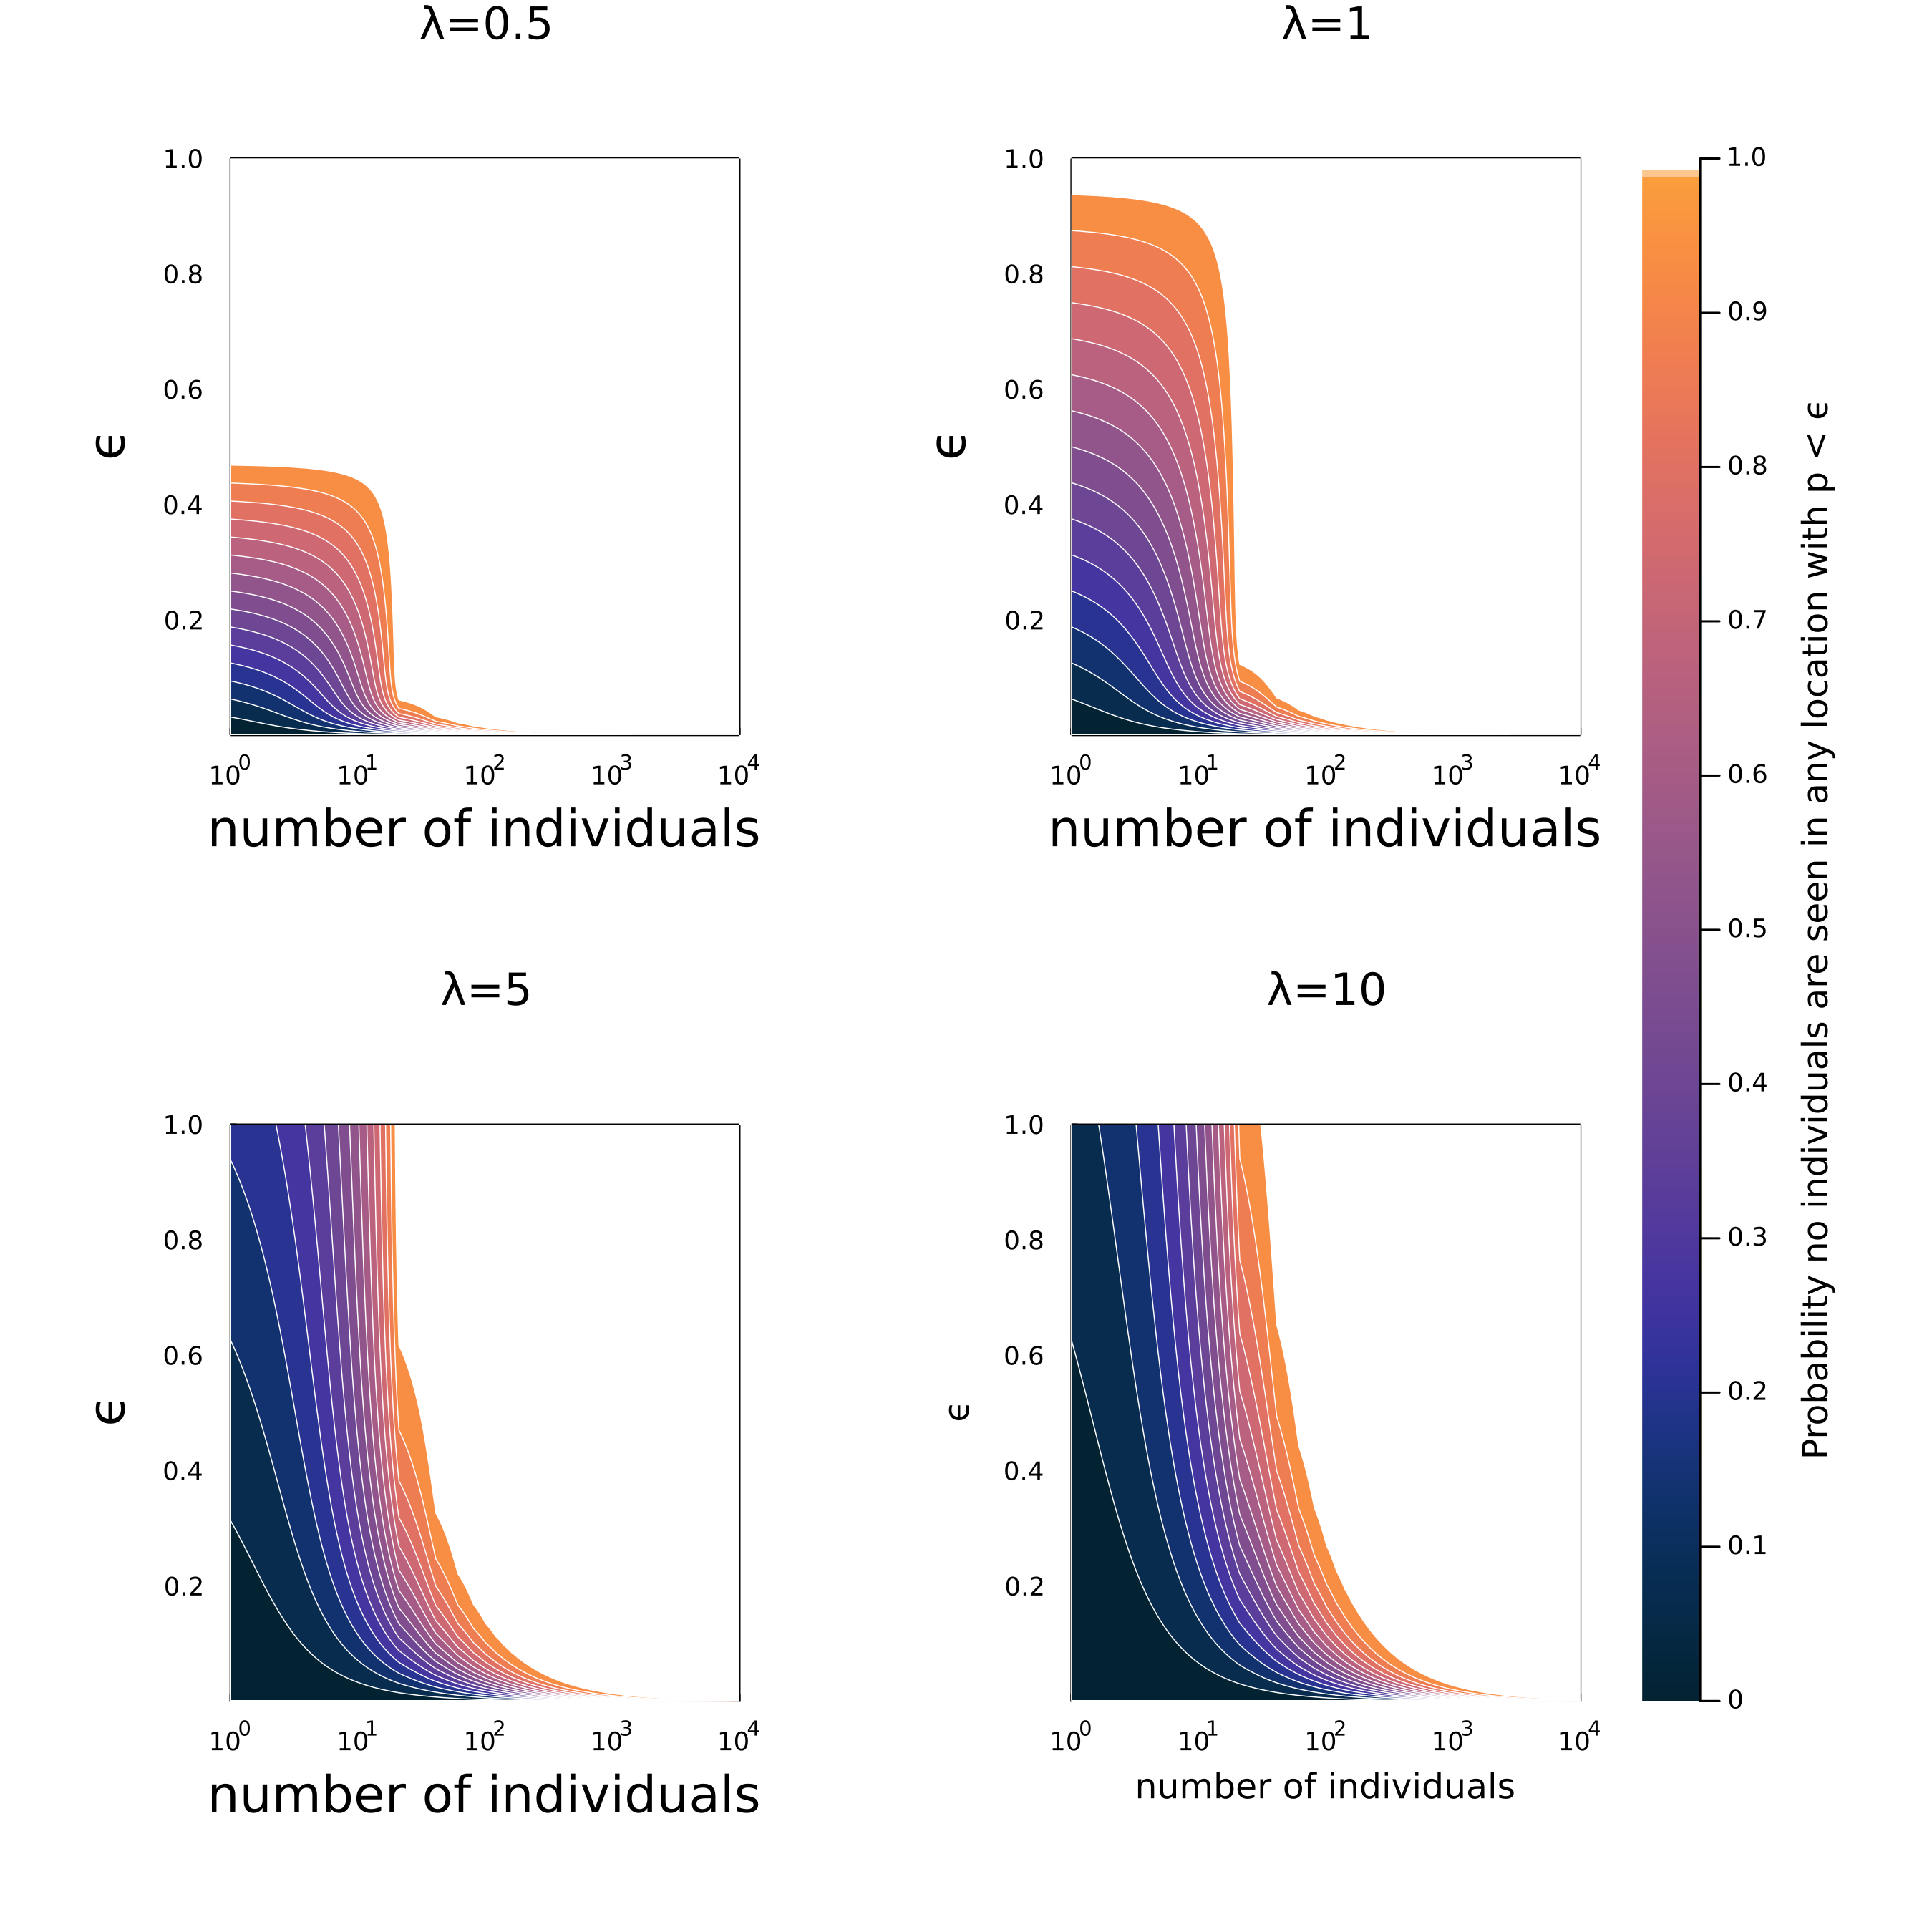
\includegraphics{./figures/neat.png}
\caption{todo}\label{fig:neato}
}
\end{figure}

As the mass of probability becomes more ``evenly spread'' across the
entire spatial domain, the probability of all individuals being observed
in locations with \(p > \epsilon\) goes down, as there are more cells
with \(p \leq \epsilon\).

\hypertarget{test-if-continuous-approx-of-space-holds-for-various-raster-sizes}{%
\subsection{Test if continuous approx of space holds for various raster
sizes}\label{test-if-continuous-approx-of-space-holds-for-various-raster-sizes}}

In this section we risk falling into the mind-projection fallacy again,
as in reality, an SDM is described by a finite \(n\)x\(m\) raster where
the values of the raster at an index \((x,y)\) and does not ``truly''
follow an exponential distribution as assumed above.

\hypertarget{an-example-use-real-data-and-make-and-sdm-and-report-different-maps-based-on-simulating-occurrence}{%
\section{An example: use real data and make and SDM, and report
different maps based on simulating
occurrence}\label{an-example-use-real-data-and-make-and-sdm-and-report-different-maps-based-on-simulating-occurrence}}

\hypertarget{conc}{%
\section{Conc}\label{conc}}

Jaynes on the mind-projection fallacy:

\begin{quote}
In studying probability theory, it was vaguely troubling to see
reference to ``Gaussian random variables,'' or ``stochastic processes,''
or ``stationary time-series,'' or ``disorder,'' as if the property of
being Gaussian, random, stochastic, stationary, or disorderly is a real
property, like the property of possessing mass or length, existing in
Nature\ldots{} As soon as the error had a definite name and description,
it was much easier to recognize. Once one has grasped the idea, one sees
the Mind Projection Fallacy everywhere; what we have been taught as deep
wisdom, is stripped of its pretensions and seen to be instead a foolish
non sequitur. The error occurs in two complementary forms, which we
might indicate thus:

A): My own imagination -\textgreater{} Real property of Nature

B): My own ignorance -\textgreater{} Nature is indeterminate
\end{quote}

``Our own ignorance implies nature is indeterminate.'' This is why we
build SDMs. Clearly the locations of the individuals of a species at any
point in time is a measurable property of the world for which there
cannot be more than one realized value. But we cannot sample this entire
thing, so we take a subset of it and aim to estimate the this latent
``species distribution'' in order to predict where one might observe a
species.

This pattern is common in the history of science. To develop on an
example raised by Jaynes---quantum mechanics has an object that much
like a species distribution model: the wave function \(\psi\) describing
the probability of observing a particle across space. A
misinterpretation of the wave function, according to Jaynes, is that
often one assumes that the distribution of where observers see a
particle is an inherent property of that particle, rather than being a
construct of human imagination created to make predictions based on the
information we have observed about that particle. The most (in)famous
example of this is likely Schrodinger's cat: often presented as the lens
that the cat is somehow \emph{both} alive and dead at the same time--- a
quintessential of the mind-projection fallacy as described above. The
state of the external world cannot be assumed indeterminate for the sole
reason that we lack the information to fully describe it. This is
equivalent to saying if one is in New York, then for oneself London
becomes a multiverse of the possible worlds which are only realized upon
one's return.

Is ``probability'' is a fixed property of nature rather than an
abstraction used describe what we can say about a system given a set of
information? me, personally, i don't know.

\hypertarget{references}{%
\section{References}\label{references}}

\end{document}
